\section{DINOv3 on Geospatial Data}
\label{sec:satellite}
Our self-supervised learning recipe is generic and can be applied to any image domain. In this section, we showcase this universality by building a DINOv3 7B model for satellite images, which have very different characteristics (\eg object texture, sensor noise, and focal views) than the web images on which DINOv3 was initially developed.

\subsection{Pre-Training Data and Benchmarks}


Our satellite DINOv3 7B model is pre-trained on \SATdataset, a dataset of 493 millions of $512\times512$ images sampled randomly from Maxar RGB ortho-rectified imagery at 0.6 meter resolution.
We use the exact same set of hyper-parameters that are used for the web DINOv3 7B model, except for the RGB mean and std normalization that are adapted for satellite images, and the training length. 
Similar to the web model, our training pipeline for the satellite model consists of 100k iterations of initial pre-training with global crops ($256\times 256$), followed by 10k iterations using Gram regularization, and finalized with 8k steps of high resolution fine-tuning at resolution $512$. 
Also similar to the web model, we distill our 7B satellite model into a more manageable ViT-Large model to facilitate its use in low-budget regime.

We evaluate DINOv3 satellite and web models on multiple earth observation tasks. For the task of global canopy height mapping, we use the Satlidar dataset described in \cref{app:exp-details:geospatial}, which consists of one million $512\times 512$ images with LiDAR ground truths split into train/val/test splits with ratios 8/1/1. The splits include the Neon and S\~{a}o Paulo dataset used by \citet{tolan2024very}.
For national-scale canopy height mapping, we evaluate on Open-Canopy \citep{fogel2025open}, which combines SPOT 6-7 satellite imagery and aerial LiDAR data over 87,000 km$^2$ across France.
Since images in this dataset have 4 channels including the additional infra-red (IR) channel, we adapt our backbone by taking the average of the three channels in the weights of the patch embed module and adding it to the weights as the fourth channel.
We trained a DPT decoder on $512\times 512$ crops of images resized to 1667 to match the Maxar ground sample resolution. %



\begin{table}[t]
  \centering
  \small
  \caption{Evaluation of different backbones for high-resolution canopy height prediction. All models are trained with a DPT decoder. Results are presented either for experiments with the decoder trained on SatLidar and evaluated on IID samples (SatLidar Val) and OOD test sets (SatLidar Test, Neon and S\~{a}o Paulo), or for experiments with the decoder trained and evaluated on the Open-Canopy dataset.
  We list mean absolute error (MAE) and the block $R^2$ metric from \citet{tolan2024very}.
  For completeness, we additionally evaluate the original decoder of \citet{tolan2024very} that was trained on Neon dataset (denoted by $^\ast$).}
  \label{tab:canopy}
  \setlength{\tabcolsep}{4pt}
  \begin{tabular}{@{}ll c cc c cc cc cc c c@{}}
    \toprule
    \multirow{3}{*}{Method} & \multirow{3}{*}{Arch.} & & \multicolumn{9}{c}{SatLidar} & & \multirow{2}{*}{Open Canopy} \\
    \cmidrule{4-5} \cmidrule{7-12}
    & & & \multicolumn{2}{c}{SatLidar Val} 
       & & \multicolumn{2}{c}{SatLidar Test}  
          & \multicolumn{2}{c}{Neon Test}    
          & \multicolumn{2}{c}{S\~{a}o Paulo} & & \\
        \cmidrule{4-5} \cmidrule{7-8} \cmidrule{9-10} \cmidrule{11-12} \cmidrule{14-14} 
     & & & MAE↓ & $R^2$↑ & & MAE↓   & $R^2$↑ & MAE↓   & $R^2$↑ & MAE↓   & $R^2$↑ & & MAE↓ \\
    \midrule
    \citet{tolan2024very}$^\ast$  & ViT-L 
       & & 2.8    & 0.86   
       & & 4.0    & 0.61   
         & 2.7    & 0.73   
         & \textbf{5.4}    & 0.42   
         & & ---  \\
    \citet{tolan2024very}  & ViT-L 
       & & 2.4    & 0.90   
       & & 3.4    & 0.81   
         & 2.9    & 0.69   
         & \textbf{5.4} & 0.48  
         & & 2.42 \\
    DINOv3 Web  & ViT-7B 
       & & 2.4    & 0.90   
       & & 3.6    & 0.74   
         & 2.7    & 0.75
         & 5.9    & 0.34   
         & & 2.17  \\
    DINOv3 Sat  & ViT-L
       & & \textbf{2.2} & 0.91 
       & & \textbf{3.2} & 0.81 
         & \textbf{2.4} & \textbf{0.81}  
         & 5.8    & 0.42 
         & & 2.07 \\
    DINOv3 Sat  & ViT-7B 
       & & \textbf{2.2} & \textbf{0.92} 
       & & \textbf{3.2} & \textbf{0.82} 
         & 2.6 & 0.74  
         & 5.5    & \textbf{0.51} 
         & & \textbf{2.02} \\
    \bottomrule
  \end{tabular} %
\end{table}

Semantic geospatial tasks are assessed with GEO-Bench \citep{lacoste2023geo}, which comprises six classification and six segmentation tasks spanning various spatial resolutions and optical bands. The GEO-Bench tasks are diverse, including the detection of rooftop-mounted photovoltaic systems, classifying local climate zones, measuring drivers of deforestation, and detecting tree crowns. For high-resolution semantic tasks, we consider the land cover segmentation dataset LoveDA \citep{wang2022lovedaremotesensinglandcover}, the object segmentation dataset iSAID \citep{zamir2019isaidlargescaledatasetinstance}, and the horizontal detection dataset DIOR \citep{li2020object}. 

\subsection{Canopy Height Estimation}

Estimating canopy height from satellite imagery is a challenging metric task, requiring accurate recovery of continuous spatial structure despite random variations in slope, viewing geometry, sun angle, atmospheric scattering, and quantization artifacts.
This task is critical for global carbon monitoring and for forest and agriculture management \citep{harris2021}.
Following \citet{tolan2024very}, the first work to leverage a SSL backbone trained on satellite images for this task, we train a DPT head on top of frozen DINOv3 on the SatLidar1M training set, then evaluate it on i.i.d.~samples on SatLidar1M validation set as well as out-of-distribution test sets including SatLidar1M test, Neon and Sao Paulo.
We additionally train and evaluate on the Open-Canopy dataset. 

\omitme{revise text if removing Sao Paulo}
\paragraph[Results]{Results (\cref{tab:canopy})}
We compare different SSL backbones, denoting with ``DINOv3 Sat'' the model trained the \SATdataset dataset, and with ``DINOv3 Web'' the model trained on \LVDdataset (see \cref{sec:data}).
It can be seen that DINOv3 satellite models yield state-of-the-art performance on most benchmarks.
Our 7B satellite model sets the new state of the art on SatLidar1M val, SatLidar1M test and Open-Canopy, reducing MAE from $2.4$ to $2.2$, from $3.4$ to $3.2$ and from $2.42$ to $2.02$ respectively. These results show that DINOv3 training recipe is generic and can be effectively applied out-of-the-box to other domains. 
Interestingly, our distilled ViT-L satellite model performs comparably to its 7B counterpart, achieving comparable results on SatLidar1M and Open-Canopy while faring surprisingly better on Neon test set, reaching the lowest MAE of $2.4$ compared to $2.6$ of the 7B model and $2.9$ of \citet{tolan2024very}.
Our DINOv3 7B web model reaches decent performance on the benchmarks, outperforming \citet{tolan2024very} on SatLidar1M val, Neon and Open-Canopy but stays behind the satellite model.
This highlights the strength of domain-specific pretraining for physically grounded tasks like canopy height estimation, where sensor-specific priors and radiometric consistency are important.


\subsection{Comparison to the Earth Observation State of the Art}




\begin{table}[t]
    \centering
    \footnotesize
    \caption{
    Comparison of our DINOv3 models against strong baselines DOFA~\citep{xiong2024neural}, Prithvi-v2~\citep{szwarcman2024prithvi}, and \citet{tolan2024very} in Geo-Bench tasks. While Privthi-v2 and DOFA leverage all available optical bands, our models achieve significantly better performance with only RGB inputs.\looseness-1
    }
    \label{tab:Geobench}
    \begin{subtable}{\linewidth}
        \centering
        \caption{Classification tasks.}
        \vspace{-0.4em}
        \setlength{\tabcolsep}{4pt}
        \begin{tabular}{@{}lcccccccccc@{}}
            \toprule
            Method & Arch. & FT & Bands & m-BEnet & m-brick-kiln & m-eurosat & m-forestnet & m-pv4ger & m-so2sat & Mean \\
             \midrule
           DOFA  & ViT-L &\orangefire & all & 68.7 & 98.4 & 96.6 & 55.7 & 98.2 & 61.6 &  79.9 \\
           Best of Prithvi-v2  & ViT-L/H& \orangefire & all & 71.2  & {\bf98.8} & 96.4 & 54.1 & {98.1} & 59.1 & 79.6\\
           \citet{tolan2024very} & ViT-L & \bluesnow & RGB & 66.0 & 97.1 & 95.2 & 56.3 & 94.3  & 58.1 & 77.8\\
           DINOv3 Sat & ViT-L &\bluesnow & RGB & 73.0 & 96.5 & 94.1 & 60.6 & 96.0 & 57.4 & 79.6 \\
           DINOv3 Sat & 7B &\bluesnow & RGB &  74.0 & 97.2 & 94.8 & {\bf 62.3} & 96.1 & 62.1 & 81.1 \\ %
           DINOv3 Web & 7B & \bluesnow & RGB & {\bf 74.6} & 97.7& {\bf 97.0} & 57.9 & {\bf 98.3} & {\bf 63.8} & {\bf 81.6}  \\
            \bottomrule
        \end{tabular} %
     \end{subtable}
     
     \vspace{1em}
     \begin{subtable}{\linewidth}
        \centering
        \caption{Segmentation tasks.}
        \vspace{-0.4em}
        \setlength{\tabcolsep}{2pt}
         \begin{tabular}{@{}lcccccccccc@{}}
            \toprule
            Method & Arch. & FT & Bands & m-cashew$^{*}$ & m-chesapeake & m-NeonTree & m-nz-cattle & m-pv4ger-seg & m-SA-crop & Mean  \\
            \midrule
           DOFA & ViT-L&\orangefire& all & 81.2 &61.6  & 58.5 & 77.4 & 95.1 & 35.7 & 68.3\\
           Best of Prithvi-v2  & ViT-L/H& \orangefire & all& 90.2 & 69.4 & 59.1 & 81.0 & 95.3 & {\bf41.9} & 72.8 \\
           \citet{tolan2024very} & ViT-L & \bluesnow& RGB& 92.8 &73.7 & 58.1& 83.1& 94.7& 35.1 & 72.9\\
           DINOv3 Sat & ViT-L & \bluesnow & RGB & 94.2 & 75.6	& 61.8 & \textbf{83.7} & 95.2 & 36.8 & 74.5 \\ 
           DINOv3 Sat & 7B & \bluesnow & RGB & 94.1 & {\bf76.6} & 62.6 &  83.4 & 95.5 & 37.6 & 75.0 \\
           DINOv3 Web & 7B & \bluesnow & RGB & {\bf 96.0} & 76.5& {\bf 66.4}& {\bf 83.7} & {\bf 95.9}& 36.8& {\bf 75.9}  \\
            \bottomrule
        \end{tabular} %
    \end{subtable}
    \begin{flushleft}
        \vspace{-0.2em}
        {\footnotesize $^{*}$\textit{Conversion to 6 classes following \citet{szwarcman2024prithvi}.}}
    \end{flushleft}
\end{table}

We compare the performance of different methods for Earth observation tasks in~\cref{tab:Geobench} and~\cref{tab:sat_highres}.
The frozen DINOv3 satellite and web models set new state-of-the-art results on 12 out of 15 classification, segmentation, and horizontal object detection tasks. Our Geo-Bench results surpass prior models, including Prithvi-v2~\citep{szwarcman2024prithvi} and DOFA~\citep{xiong2024neural}, which use 6+ bands for Sentinel-2 and Landsat tasks, as well as task-specific fine-tuning (\cref{tab:Geobench}).
Despite using a frozen backbone with RGB-only input, the DINOv3 satellite model outperforms previous methods on the three unsaturated classification tasks and on five of six segmentation tasks. Interestingly, the DINOv3 7B web model is very competitve on these benchmarks.
It achieves comparable or stronger performance on many GEO-Bench tasks as well as on large-scale, high-resolution remote sensing benchmarks for segmentation and detection.
As shown in \cref{tab:Geobench} and \cref{tab:sat_highres}, the frozen DINOv3 web model establishes new leading results Geo-Bench tasks as well as for segmentation and detection tasks on the LoveDA and DIOR datasets. 












These findings have broader implications for the design of geospatial foundation models.
Those have recently emphasized heuristic techniques such as multitemporal aggregation, multisensor fusion, or incorporating satellite-specific metadata \citep{brown2025alphaearthfoundationsembeddingfield, feng2025tesseratemporalembeddingssurface}.
Our results show that general-purpose SSL can match or exceed satellite-specific approaches for tasks that depend on precise object boundaries (segmentation or object detection). 
This supports emerging evidence finding that domain-agnostic pretraining can offer strong generalization even in specialized downstream domains \citep{lahrichi2025selfsupervisedpretrainingsatelliteimagery}.  

Collectively, our results suggest task-dependent benefits of domain-specific pretraining.
The DINOv3 satellite model excels in metric tasks like depth estimation, leveraging satellite-specific priors.
In contrast, the DINOv3 web model achieves state-of-the-art results on semantic geospatial tasks through diverse, universal representations.
The complementary strengths of both models illustrate the broad applicability and effectiveness of the DINOv3 SSL paradigm. %


\omitme{
}


\begin{figure}[t]
    {\small%
        \begin{tabular}{@{}c@{\hspace{0.64em}}c@{\hspace{0.64em}}c@{\hspace{0.64em}}c@{\hspace{0.64em}}c@{}}
        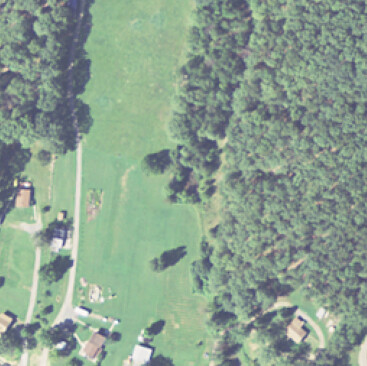
\includegraphics[width=0.19\linewidth]{figures/satellite/img.lr.jpg}&
        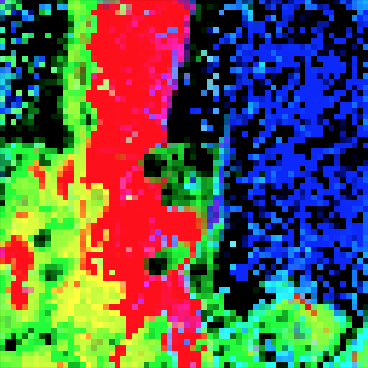
\includegraphics[width=0.19\linewidth]{figures/satellite/dinov2.png}&
        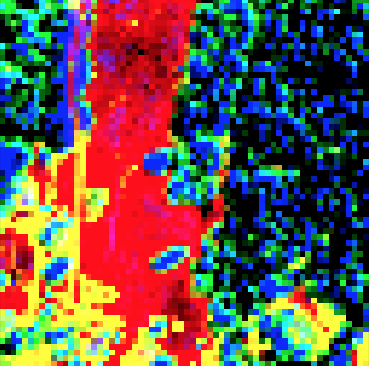
\includegraphics[width=0.19\linewidth]{figures/satellite/dinov3.png}&
        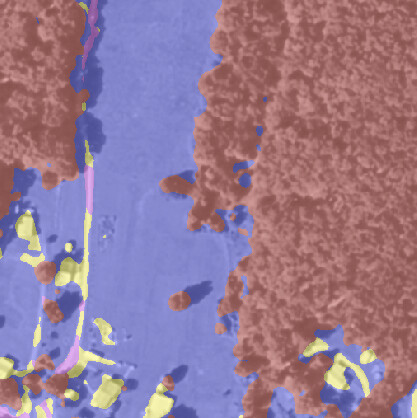
\includegraphics[width=0.19\linewidth]{figures/satellite/seg2.lr.jpg}&
        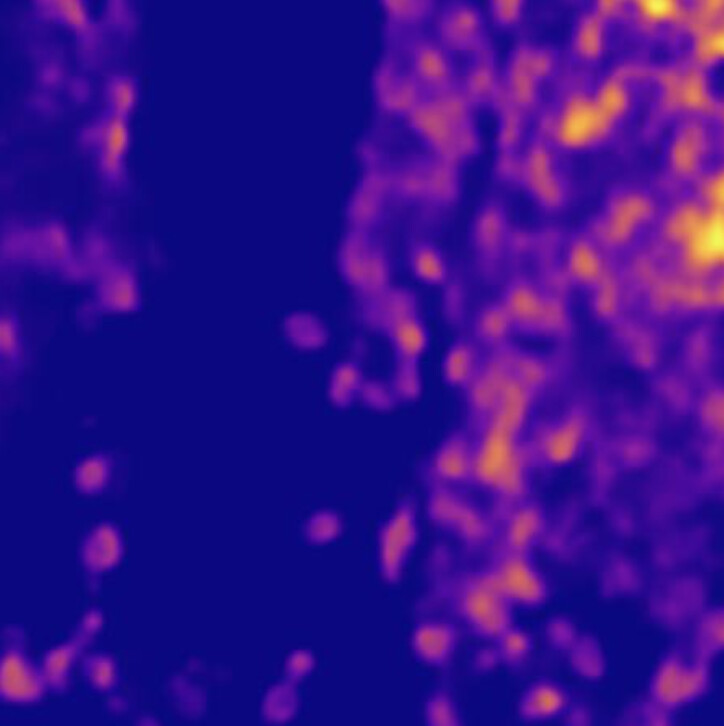
\includegraphics[width=0.19\linewidth]{figures/satellite/chm.lr.jpg}\\
        Img in Chesapeake & PCA DINOv2 & PCA DINOv3 & Segmentation v3 & Canopy height v3 \\
        \end{tabular}
    }
    \caption{
        Illustration of versatile applications in remote sensing made possible by a single DINOv3 model. The PCA on DINOv3 features shows finer details than DINOv2. The segmentation map was computed using only GEO-Bench chesapeake labels. The canopy height model decoder was trained on the Open-Canopy dataset using 4 channels (RGB + InfraRed), while inference was performed on RGB channels only. 
    }
    \omitme{
        \hl{[to do: update with the new model]}
    } 
    \omitme{using /home/coupriec/segmentation_viz.ipynb or /home/coupriec/lavida/segmentation_viz.ipynb on CW}
    \label{fig:satfig}
\end{figure}


 \begin{table}[t]
     \centering
     \small
     \caption{We compare the performance of DINOv3 to state-of-the-art models Privthi-v2~\citep{szwarcman2024prithvi}, BillionFM~\citep{Cha_2024} and SkySense V2~\citep{zhang2025skysense} for high resolution semantic geospatial tasks. We report mIoU for the segmentation datasets LoveDA (1024$\times$) and iSAID (896$\times$), and mAP for the detection dataset DIOR ($800\times$).}
     \label{tab:sat_highres}
      \begin{tabular}{@{}llc c c c c@{}}
        \toprule
          Method & Arch. & FT && LoveDA & iSAID & DIOR \\%Depth on Open-Canopy \\
          \midrule
           \multirow{2}{*}{Prev. SotA} & & \multirow{2}{*}{\orangefire} && BillionFM, ViT-G  & SkySense V2, Swin-G$^\ast$ & SkySense V2, Swin-G$^\ast$ \\%PVTv2 ViT-L\\ 
            & & && 54.4  & \textbf{71.9} & 79.5 \\%& 2.52 \\ 
          \midrule
          Decoder Arch. & & && UPerNet & UPerNet & Faster-RCNN \\%& DPT\\
          Privthi-v2 & ViT-H &  \orangefire && 52.2 &  62.8  & --- \\%& - \\
          DINOv3 Sat  & ViT-L & \bluesnow  &&   54.4 &  62.9  & 72.7 \\
          DINOv3 Sat  & ViT-7B & \bluesnow  &&  55.3  &  64.8  & 76.6 \\%&  {\bf 2.02} \\ %
          DINOv3 Web & ViT-7B & \bluesnow && \textbf{56.2} & 71.4 \omitme{71.2-71.6}  & {\bf 80.5} \\%& 2.17 \\ 
          \bottomrule
      \end{tabular}
    \begin{flushleft}
        {\footnotesize $^\ast$\textit{Uses modified DINOv2 SSL with supervised pretraining alignment on OpenStreetMap, reporting +0.8 mIoU on iSAID.}}
    \end{flushleft}
 \end{table}












\begin{figure}[t]
    \centering
    \begin{tabular}{cccc}
         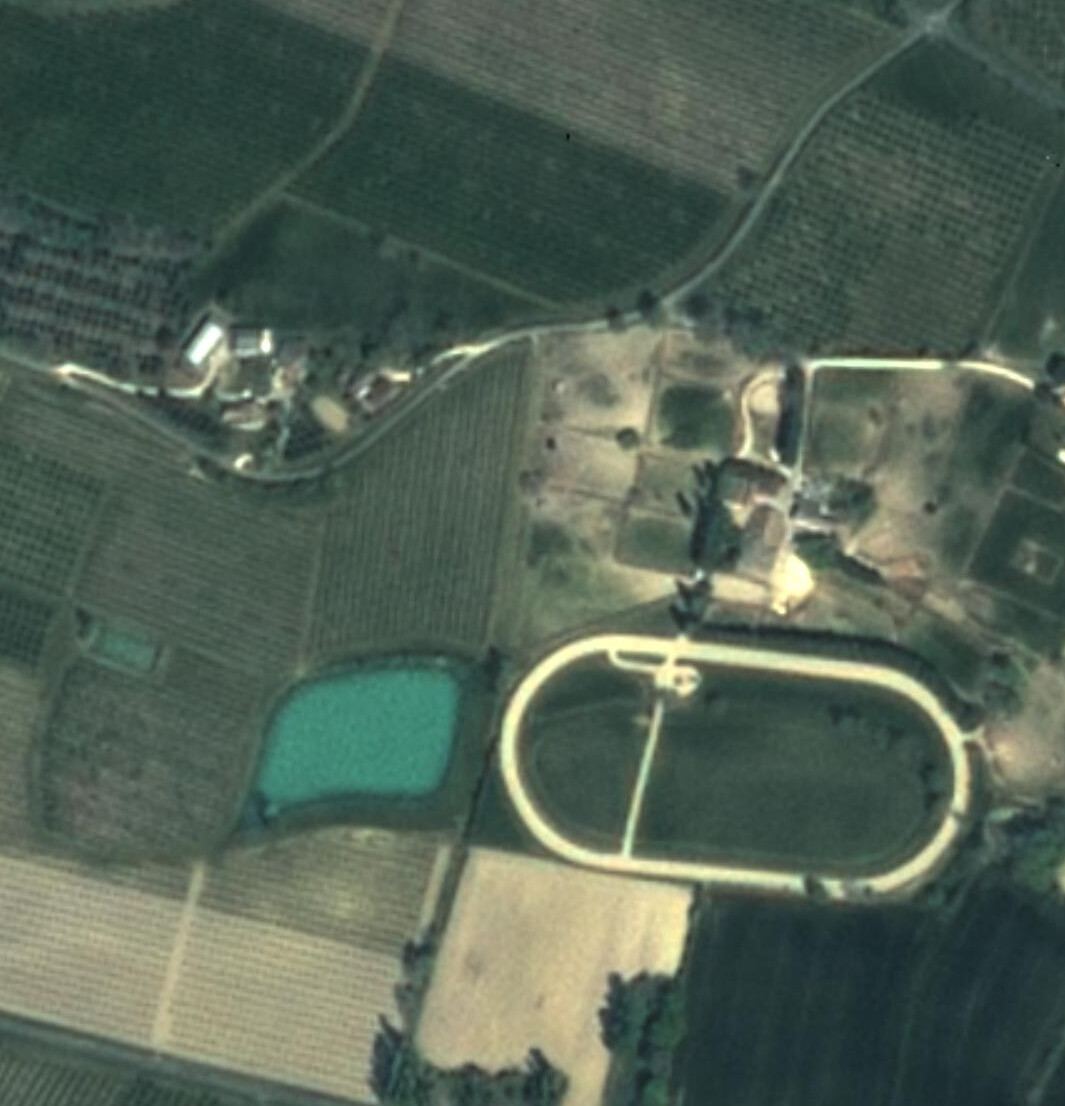
\includegraphics[width=0.22\linewidth]{figures/satellite/img12.lr.jpg}&
         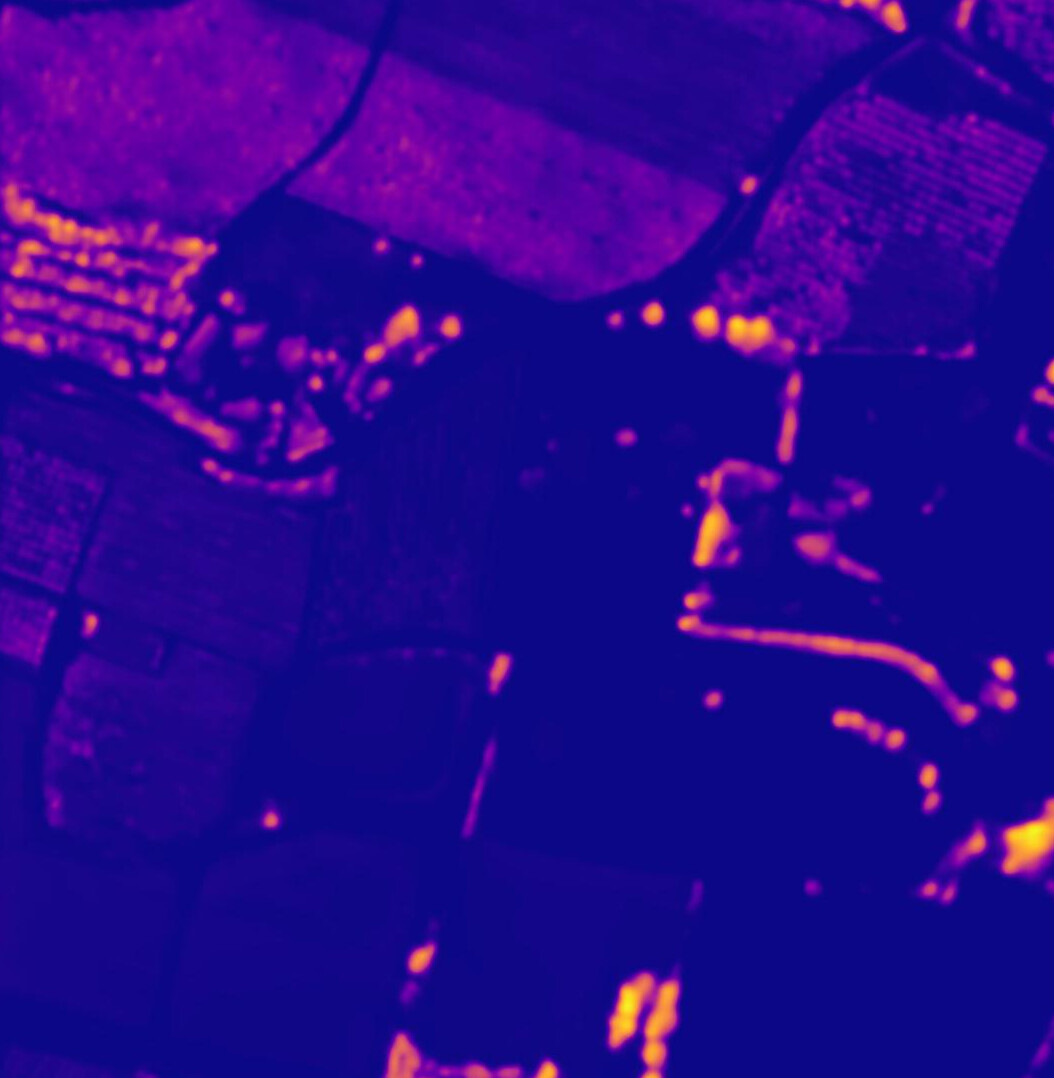
\includegraphics[width=0.22\linewidth]{figures/satellite/tolan12.lr.jpg}&
         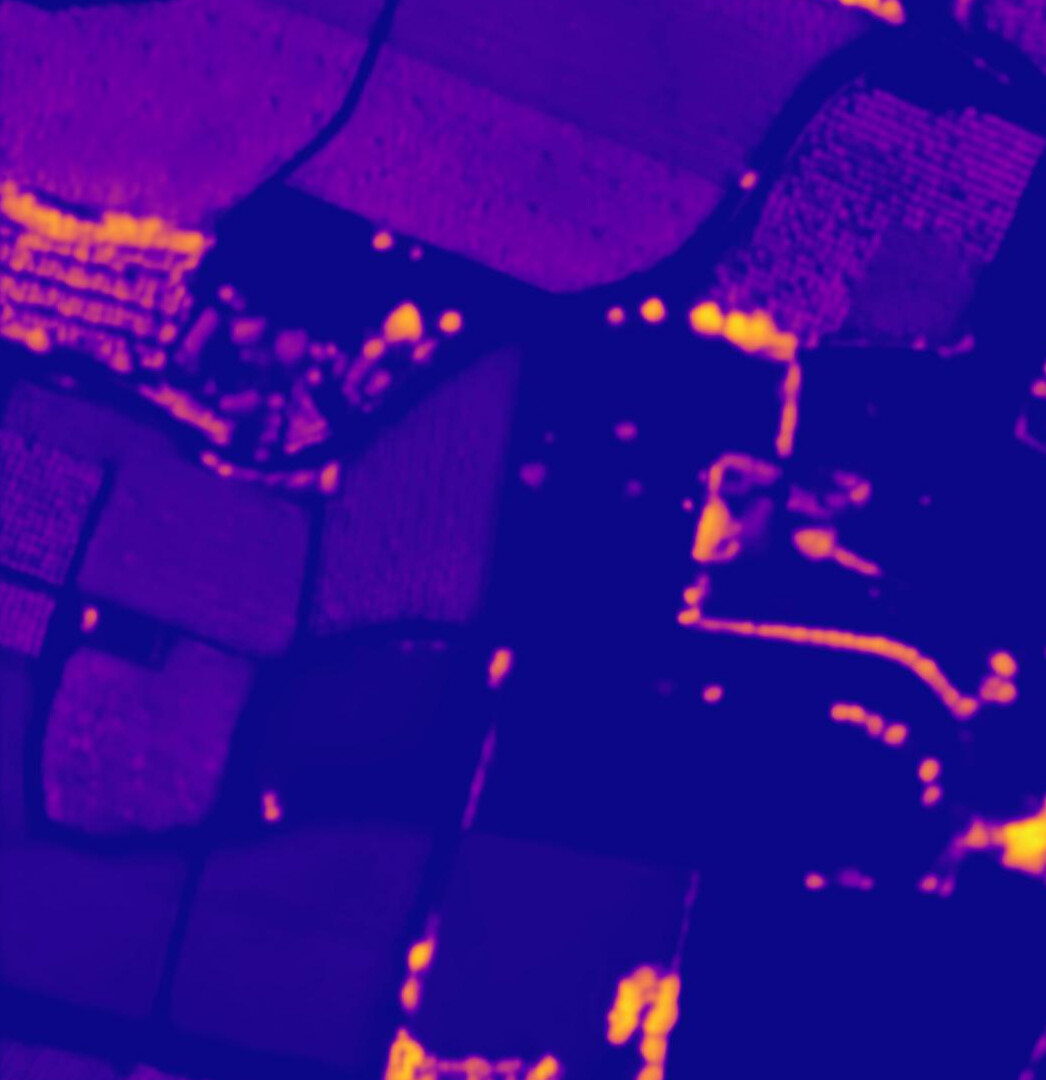
\includegraphics[width=0.22\linewidth]{figures/satellite/chm12.lr.jpg}&
         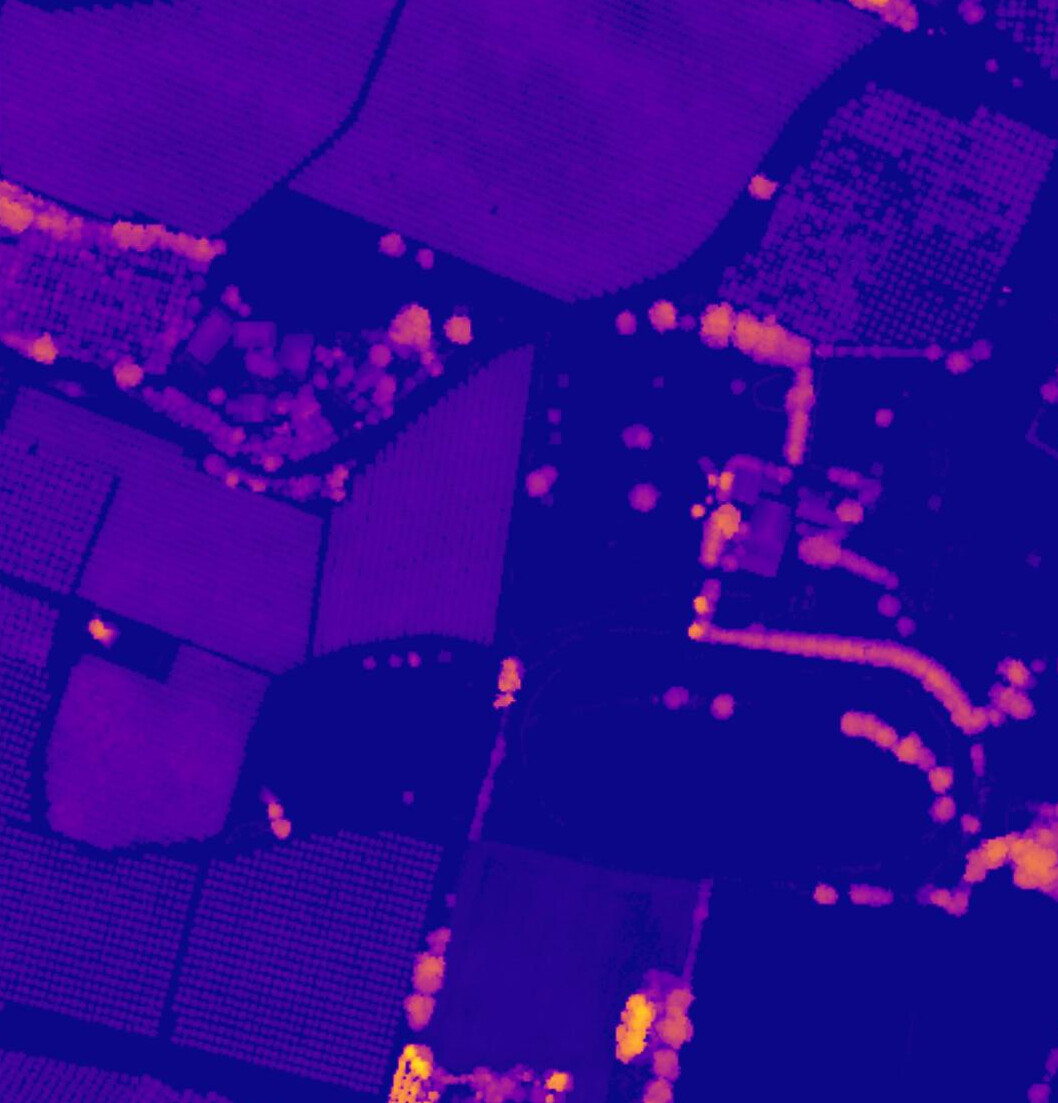
\includegraphics[width=0.22\linewidth]{figures/satellite/gt12.lr.jpg}\\
         Image from OpenCanopy& Improved Tolan et al.& DINOv3 SAT-493M & Ground Truth\\ 
    \end{tabular}
    \caption{A qualitative comparison of the DINOv3 7B satellite model to \citet{tolan2024very} on the Open Canopy dataset. For both models, the decoder is trained on 448$\times$448 input images. It can be seen that DINOv3 produces more accurate maps, for example the accurate height for the trees on the field.}
    \label{fig:placeholder}
\end{figure}
